\documentclass[12pt]{article}
\usepackage[english]{babel}
\usepackage[table,xcdraw]{xcolor}
\usepackage{booktabs}
\usepackage{tabularx}
\usepackage{enumerate}
\usepackage{graphicx}
\usepackage[section]{placeins}
\usepackage{float}
\usepackage{url}
\usepackage{wrapfig}
\usepackage[toc,page]{appendix}
\usepackage{caption}
\usepackage{enumitem}
\usepackage[style=numeric-comp, sorting=none]{biblatex}
\usepackage{pdflscape}
\usepackage{adjustbox}
\usepackage{csquotes}
\usepackage{hhline} % for double lines
\usepackage{listings}
\usepackage{hyperref}

\captionsetup{justification=centering}

\graphicspath{{images/}}
\bibliography{refs.bib}

\begin{document}

\begin{titlepage}

\newcommand{\HRule}{\rule{\linewidth}{0.5mm}} % Defines a new command for the horizontal lines, change thickness here

\center % Center everything on the page
 
%----------------------------------------------------------------------------------------
%	HEADING SECTIONS
%----------------------------------------------------------------------------------------

\textsc{\LARGE Universitat Politècnica de Catalunya}\\[1.5cm] % Name of your university/college
\textsc{\Large Algorithms, Data Structures and Databases}\\[0.5cm] % Major heading such as course name

%----------------------------------------------------------------------------------------
%	TITLE SECTION
%----------------------------------------------------------------------------------------

\HRule \\[0.4cm]
{ \huge \bfseries Deliverable 1}\\[0.4cm] % Title of your document
\HRule \\[1.0cm]
 
%----------------------------------------------------------------------------------------
%	AUTHOR SECTION
%----------------------------------------------------------------------------------------

\begin{minipage}{0.53\textwidth}
\large
\centering
\emph{Autors}\\
Aguilera Pilo \textsc{Carles}\\
Delgado Jimenez \textsc{Joel}\\
Vilella Jam \textsc{Oriol}\\
\end{minipage}
~
\begin{minipage}{0.4\textwidth}
\end{minipage}\\[2cm]

% If you don't want a supervisor, uncomment the two lines below and remove the section above
%\Large \emph{Author:}\\
%John \textsc{Smith}\\[3cm] % Your name

%----------------------------------------------------------------------------------------
%	DATE SECTION
%----------------------------------------------------------------------------------------

{\large \today}\\[2cm] % Date, change the \today to a set date if you want to be precise

%----------------------------------------------------------------------------------------
%	LOGO SECTION
%----------------------------------------------------------------------------------------


\includegraphics[scale=0.3]{logo-upc.png}\\[1cm]
 
%----------------------------------------------------------------------------------------

\vfill % Fill the rest of the page with whitespace

\end{titlepage}

\newpage

\tableofcontents

\newpage

\pagenumbering{arabic}

\newpage

\section{Instructions}

README.md

\newpage

\section{Context \& Data}

\subsection{Context}
The domain chosen for this is within the healthcare sector, specifically focusing on the detection and analysis of \textbf{skin cancer}.

We believe the current exponential growth of technology offers significant potential for application across multiple sectors, particularly in health and human well-being. This justifies our choice of domain: the development of technological tools aimed at the prediction and detection of skin cancer.

In recent years, the incidence of this disease has increased significantly, primarily due to greater public sun exposure. We therefore consider it essential to pursue data-driven and AI-based solutions that contribute to the prevention and early diagnosis of skin cancer.

As an academic project, we acknowledge this is an initial approximation. There is clear scope for future improvements, particularly concerning the model's accuracy and the quality of the data employed.

\subsection{Data}

The data for this project were primarily sourced from \textbf{Kaggle}, one of the biggest platforms in the Data Science community. This was complemented with information obtained from other open sources, such as informational websites, notably \textbf{Wikipedia}.

This are the datasets used for our project:
\begin{enumerate}
    \item \href{https://huggingface.co/datasets/abaryan/ham10000_bbox}{HAM10000 Dataset}: This dataset forms the visual part of our project. The HAM10000 dataset is a very famous and widelly used public collection of dermatoscopic images of common skin lesions, including various types of skin cancer. We load the dataset and since we can't handle all the images from the dataset, because the pipeline will be very slow, we obtain a sample of 100 images which is more than enough. This images serve as the image types of data and will be used to generate embeddings to perform similarity searches across modalities.

    \item Textual Data: This dataset proviedes the descriptive knowledge base for our project. We have implemented a \textbf{Web Scrapper} in order to scrape articles directly from Wikipedia, given some target key topics. The topics we have defined are Skin Cancer, Melanoma, Basal Cell Carcinoma, Squamous Cell Carcinoma and Actinic Keratosis. This topics can be changed at any time but the only condition is that they have to appear as a Wikipedia page. Otherwise, the scrapping will fail and it will not produce any text. 
    
    The web scrapper downloads the contents of these pages, cleans the raw HTML, and removes unnecessary elements like citation brackets. This generates our dataset which is several .txt files, one for each topic. 
    
    This text represents the descriptive modality. The embeddings generated from the text will be matched across all the embeddings we generate from the other datasets. This allows a user to search for "information about basal cell carcinoma" and get back not only this text but also related images and even audio.

    \item \href{https://huggingface.co/datasets/Moaaz55/skin_cancer_questions_answers}{Audio Data}: This is our third and last modality for this project, representing information as spoken language. In this dataset is a two-step process. We first get the content from a Hugging Face dataset containing questions and answers about skin cancer. Then, instead of using this data as text, we sample 100 of the answers from the dataset, we use a \textbf{text-to-speech} (TTS) engine to synthesize these text answers into audio. And finally we save this as individual .wav files. This creates a dataset of spoken explanations. This will allow our system to work with audio as a distinct modality. We -will generate embeddings out of this audio in order to perform similarity searches across modalities.
\end{enumerate}

\section{Data Management Backbone}

This section describes the project's data zones and the design decisions implemented for data handling and processing.

We have employed \textbf{MinIO} as our object storage system, creating a separate bucket for each layer or zone of the project. All objects are first loaded into the Temporal Landing Zone in their raw, original format, with no structure or pre-processing. The objective of this layer is to ensure rapid and complete data ingestion.

In the other layers, the buckets are organized and structured by data modality (images, text and audio). This approach allows us to maintain a clear, consistent, and more manageable data structure.

This layered architecture enables us to effectively track the data pipeline's evolution and visualitze the transformations applied to the data thoughout the entire process.

\subsection{Software Architecture}

\subsection{Landing Zone}

This project layer, the \textbf{Landing Zone}, is divided into two distinct sub-zones: the Temporal Zone and the Persistent Zone.

The first, the \textbf{Temporal Zone}, serves as the initial data ingestion or staging area. All objects are loaded here in their raw, original format, without any transformation.

The secon, the \textbf{Persistent Zone}, is where we begin to structure and organize the data. In this phase, we classify objects based on their modality (images, text or audio) and store them in their corresponding locations.

This initial organization ensures the data is correctly partitioned and prepared for subsequent processing stages.

\subsubsection{Temporal Zone}

As explained in the introductory section, this phase involves loading data from our various origin sources directly into MinIO. This ingestion allows us to capture all data within the bucket in its original, unaltered format.

\begin{figure}[H]
    \centering
    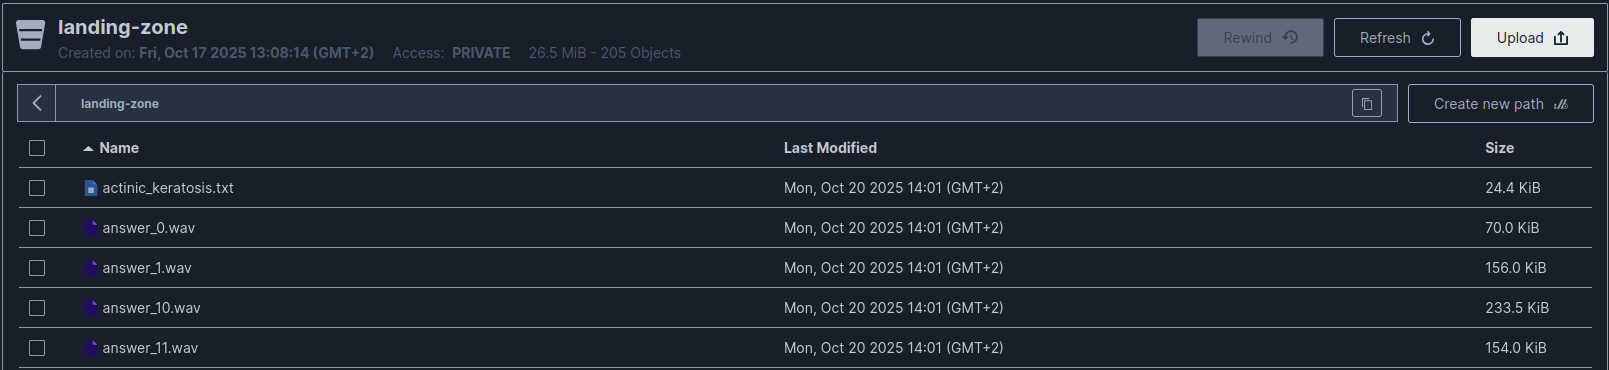
\includegraphics[width=1\linewidth]{temporal.png}
    \caption{Temporal Landing Zone}
    \label{fig:temporal}
\end{figure}

\subsubsection{Persistent Zone}

In this layer, we organized the objects and elements to simplify subsequent management and processing. To achieve this, we created a separate folder for each data type: one for images, one for text, and another for audio. This classification allows us to treat each data type differently and maintain a coherent structure with our data.


\begin{figure}[H]
    \centering
    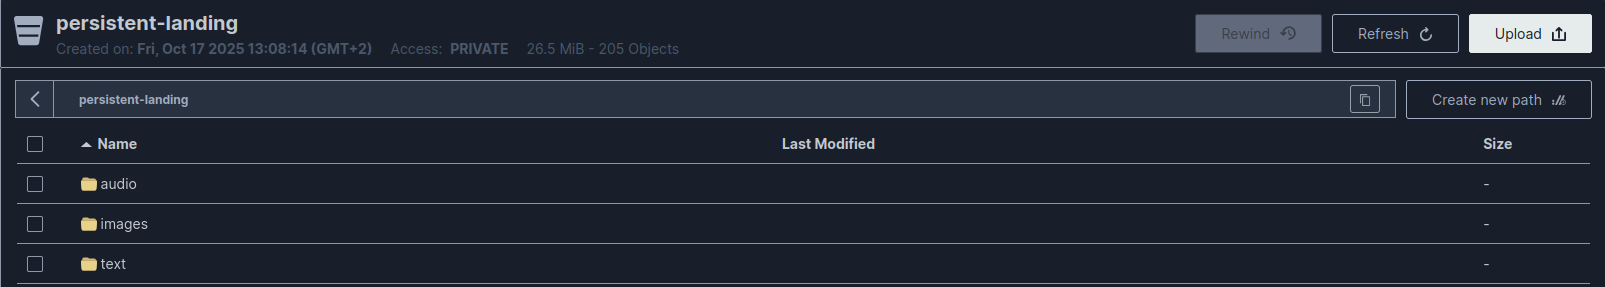
\includegraphics[width=1\linewidth]{persistent.png}
    \caption{Persistent Landing Zone}
    \label{fig:persistent}
\end{figure}

\subsection{Formated Zone}

In this layer, the data is preprocessed to ensure all elements are in a homogeneous format and a coherent structure.

Initially, we evaluated assigning a unique identifier (ID) to each object in order to facilitate traceability. However, this option was discarded after analyzing its drawbacks. This approach could have introduced duplication or inconsistency issues between different datasets. Futhermore, regenerating IDs on each load might have caused the same element to receive different identifiers at different times, making it hard to track.

It was also determined that internal IDs offered no semantic meaning and could remove the context of the initial data.

Ultimately, we opted to maintain the original filenames as the primary identifiers and ensure format consistency. All images were normalized to \textbf{.png}, texts to \textbf{.txt}, and audio to \textbf{.mp3}. These formats were chosen as the most suitable standards for each modality, simplifying future management and processing.

\begin{figure}[H]
    \centering
    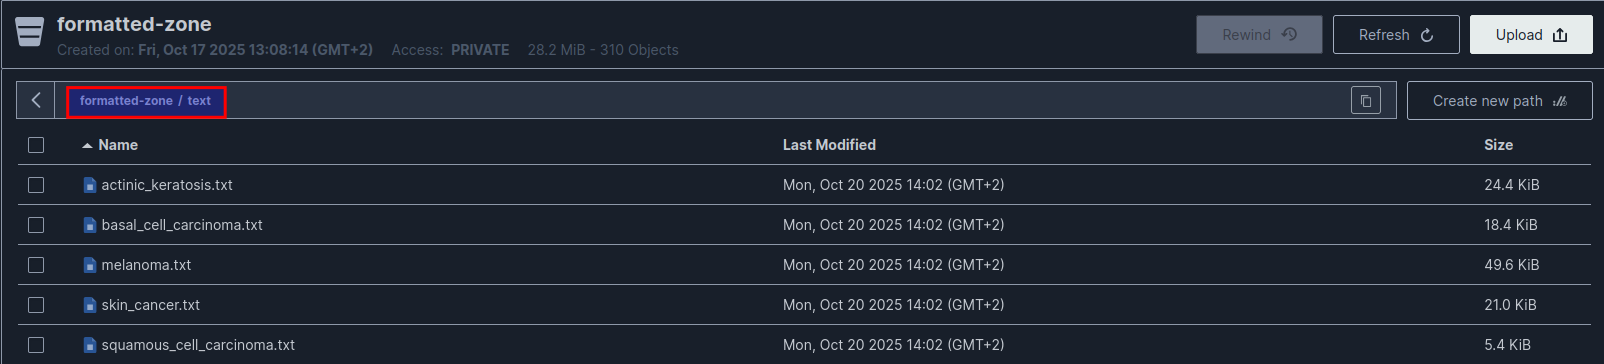
\includegraphics[width=1\linewidth]{images/formatted-text.png}
    \caption{Text format unified}
    \label{fig:placeholder}
\end{figure}

\begin{figure}[H]
    \centering
    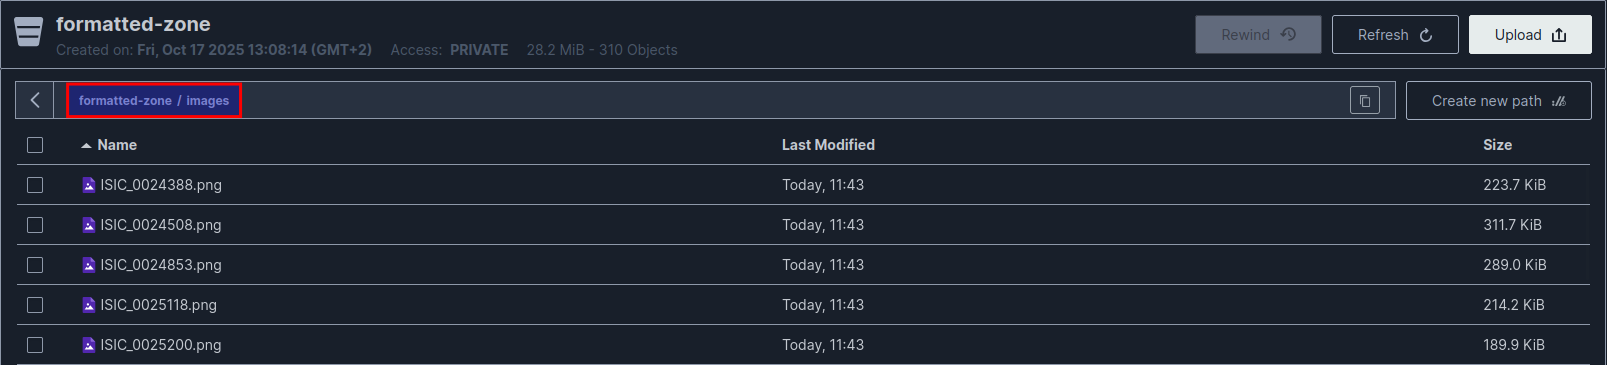
\includegraphics[width=1\linewidth]{images/formatted-images.png}
    \caption{Image format unified}
    \label{fig:placeholder}
\end{figure}

\begin{figure}[H]
    \centering
    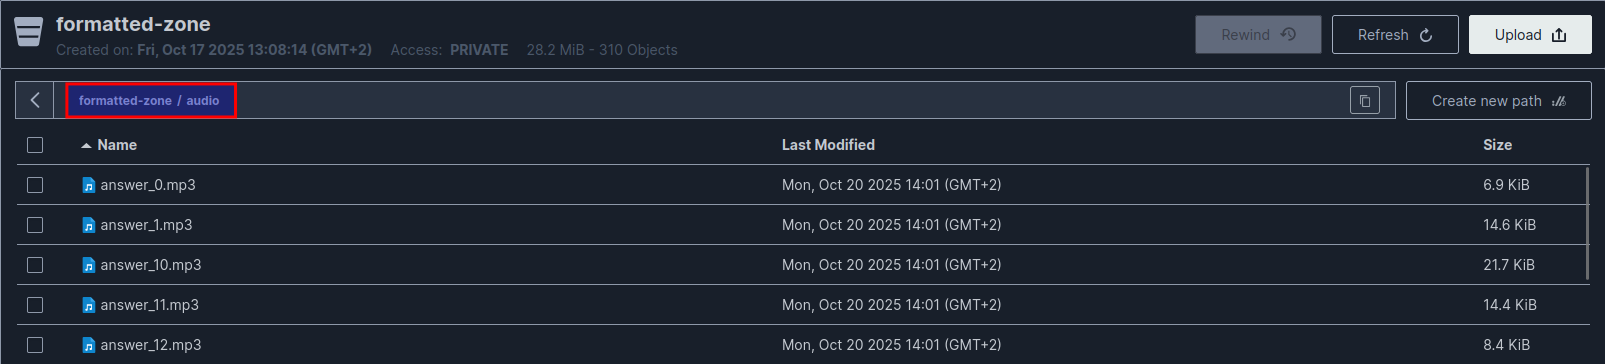
\includegraphics[width=1\linewidth]{images/formatted-audio.png}
    \caption{Audio format unified}
    \label{fig:placeholder}
\end{figure}

\subsection{Trusted Zone}

In this phase, we processed all content (images, audio and text) to ensure it was clean, standardized, and ready for use in the last stage of the pipeline.

We began with an initial analysis to identify the format and status of the data within each of three modalities. This analysis provided a general overview of the quality of the objects and characteristics, allowing us to proceed with a specific processing method for each data type.

The actions performed for each modality are detailed below.

\subsubsection{Image Processing}

Images were extracted from the Formatted Zone, processed, and then stored in the Trusted Zone. The process began by reading all image files, after which several treatments were applied to enhance visual quality.

We first did a standardization process. All images were resized to a uniform 600 by 450 pixels to ensure consistency. They were also converted to the RGB color space for compatibility with further stages of the pipeline.

Then, we also normalized the color. The brightness was increased by 10\% for clearer images, the contrast was enhanced by 15\% to highlight details and saturation was boosted by 5\% to make colors more vibrant.

Finally, a light Gaussian blur was applied to reduce digial noise. This softening was then compensated for which a sharpening filter to restore detail and maintain image clarity.

\subsubsection{Text Processing}

Text is cleaned and normalized to ensure coherence, readability, and compatibility with subsequent storage

\section{Exploitation Zone}

The primary objective of this zone is to take different types of data (images, text and audio) and convert each one into a embedding in a \textbf{unified} space.

After evaluating each model, we selected the \href{https://github.com/facebookresearch/ImageBind}{ImageBind} model because it could embed all three data types into the same space and we will not require additional models to embed the data in the different spaces. For instance, if we used different models, we would had to embed text in more than one space (one for the similarity search across texts and another for the similarity searches across other modalities). We thought this could impact the performance of our pipeline and we did the processing with one single model to achieve everything.

In the official ImageBind documentation, the standard functions for generating embeddings require a path to a file. This limitation was not suitable for our application. That would mean that we download the object from the MinIO in a temporal folder, process it and then delete it. So, what we did is to observe and understand the internals of the model and based on that, we implemented our own solution to bypass this file-path limitation.

This custom implementations allowed us to generate embeddings directly from in-memory data, which is far more suitable for our pipeline. Then, we only had to pass each of the files from the Trusted Zone into our custom implementation and insert them into the \textbf{ChromaDB} for future modal searches.

\end{document}